\section{ЗАДАНИЕ}

Составить программу -- базу знаний, с помощью которой можно определить, например, множество студентов, обучающихся в одном ВУЗе. Студент может одновременно обучаться в нескольких ВУЗах. Привести примеры возможных вариантов вопросов и варианты ответов (не менее 3-х). Описать порядок формирования ответа.

\begin{lstlisting}[caption=Текст программы]
domains
	firstname, lastname = string.
	student = student(firstname, lastname).
	nameuniversity, city = string.
	university = university(nameuniversity, city).

predicates
	learn(student, university).

clauses
	learn(student("Ivan", "Ivanov"), university("BMSTU", "Moscow")).
	
	learn(Student1, university("Coursera", "Online")) :-
	learn(Student1, university("BMSTU", "Moscow")).

	learn(student("Vasilii", "Vasiliev"), university("MSU", "Moscow")).

	learn(student("Ivan", "Popov"), university("MIFI", "Moscow")).
	
	learn(student("Petr", "Popov"), university("MIFI", "Moscow")).
	learn(student("Petr", "Popov"), university("Coursera", "Online")).

	learn(student("Petr", "Petrov"), university("MFTI", "Moscow")).
	learn(student("Petr", "Petrov"), university("Stepik", "Online")).
	
	learn(student("Vasilii", "Popov"), University) :-
	learn(student("Petr", "Popov"), University).

	learn(student("Alexander", "Ivanov"),
		university("ITMO", "Saint-Petersburg")).

	learn(student("Petr", "Ivanov"),
		university("ITMO", "Saint-Petersburg")).
	learn(student("Petr", "Ivanov"),
		university("SPBSTU", "Saint-Petersburg")).

	learn(student("Ivan", "Vasiliev"),
		university("ITMO", "Saint-Petersburg")).

	learn(student("Alexander", "Petrov"),
		university("SPBSTU", "Saint-Petersburg")).

	learn(Student2, university("Stepik", "Online")) :-
	learn(Student2, university("ITMO", "Saint-Petersburg")).
	
goal
	% learn(Student, university(Uneversity, "Online")).
	% learn(Student, university(University, "Moscow")).
	% learn(Student, university(University, "Saint-Petersburg")).
	% learn(student("Petr", "Petrov"), University).
	learn(student("Ivan", "Ivanov"), university("BMSTU", "Moscow")).
\end{lstlisting}

\subsection{Результаты работы программы}

\begin{lstlisting}[caption=Тест 1]
learn(Student, university(Uneversity, "Online")).
\end{lstlisting}

\begin{figure}[H]
    \centering
    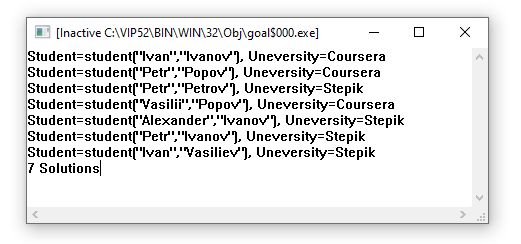
\includegraphics{img/Online.png}
    \caption{Результат теста 1}
\end{figure}

\begin{lstlisting}[caption=Тест 2]
learn(Student, university(University, "Moscow")).
\end{lstlisting}

\begin{figure}[H]
    \centering
    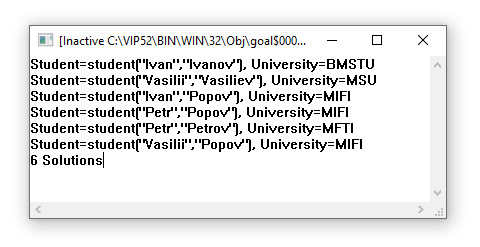
\includegraphics{img/Moscow.png}
    \caption{Результат теста 2}
\end{figure}

\begin{lstlisting}[caption=Тест 3]
learn(Student, university(University, "Saint-Petersburg")).
\end{lstlisting}

\begin{figure}[H]
    \centering
    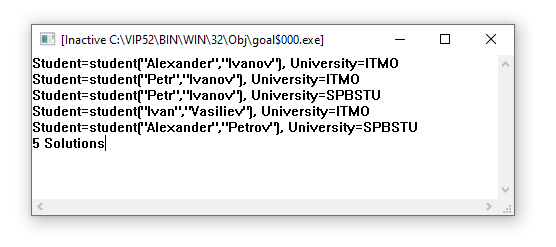
\includegraphics{img/SP.png}
    \caption{Результат теста 3}
\end{figure}

\begin{lstlisting}[caption=Тест 4]
learn(student("Petr", "Petrov"), University).
\end{lstlisting}

\begin{figure}[H]
    \centering
    
\includegraphics{img/Petr.png}
    \caption{Результат теста 4}
\end{figure}

\begin{lstlisting}[caption=Тест 5]
learn(student("Ivan", "Ivanov"), university("BMSTU", "Moscow")).
\end{lstlisting}

\begin{figure}[H]
    \centering
    
\includegraphics{img/Ivan.png}
    \caption{Результат теста 5}
\end{figure}

\section{ПРОГРАММА НА PROLOG}

С помощью термов, фактов и правил <<описываются>> знания о предметной области, то есть \textbf{база знаний}. Используя базу знаний, система Prolog будет делать логические выводы, отвечая на наши вопросы. Таким образом, \textbf{программа на Prolog представляет собой базу знаний и вопрос}.

\subsection{Переменные}

\begin{itemize}
    \item Именованная -- обозначается комбинацией символов латинского алфавита, цифр и символа подчеркивания, начинающейся с прописной буквы или символа подчеркивания (X, Student, \_X)
    \item Анонимная -- обозначается символом почеркивания (\_)
\end{itemize}

Переменные в момент фиксации утверждений в программе, обозначая некоторый неизвестный объект из некоторого множества объектов, не имеют значения. Значения для переменных могут быть установлены Prolog-системой только в процессе поиска ответа на вопрос, то есть реализации программы.

Переменные предназначены для передачи значений <<во времени и пространстве>>. Переменные в факты и правила входят только с квантором всеобщности. А в вопросы переменные входят только с квантором существования.

В процессе выполнения программы переменные могут сязываться с различными объектами -- \texbf{конкретизироваться}. Это относится только к именованным переменным. Анонимные переменные не могут быть связаны со значением.

\subsection{Структура программы}

\begin{itemize}
    \item директивы компилятора -- зарезервирвоанные символьные константы
    \item CONSTANST -- раздел описания констант
    \item DOMAINS -- раздел описания доменов
    \item DATABASE -- раздел описания предикатов внутренней базы данных
    \item PREDICATES -- раздел описания предикатов
    \item CLAUSES -- раздел описания предложений базы знаний
    \item GOAL -- раздел описания внутренней цели (вопроса)
\end{itemize}

В программе не обязательно дожны быть все разделы.

\subsection{Реализация структуры}

База знаний состоит из предложений -- CLAUSES: фактов и правил.
Каждое предложение заканчивается точкой.

\textbf{Правило имеет вид}: { \ttfamily A :- B$_1$, ..., B$_n$. } A называется \textbf{заголовком правила}, а $B_1, ..., B_n$ -- телом правила.

\textbf{Факт} -- это частный случай правила (в котором нет тела).

\textbf{Заголовок} содержит отдельное знание о предметной области, а тело содержит условия истинности этого знания. Правило называют условной истиной, а факт, не содержащий тела -- безусловной истиной.

Заголовок содержит знание о том, что между аргументами существует отношение.

\subsection{Формирование результата}

С помощью подбора ответов на запросы Prolog извлекает хранящуюся информацию. База знаний содержит истиностные знания, используя которые программа выдает ответ на запрос. Одной из особенностей Prolog является то, что при поиске ответов на вопрос, он рассматривает альтернативные варианты и находит все возможные решения -- множества значений переменных, при которых на поставленный вопрос можно онтевить <<да>>.
